\section{Performance} \label{sec:res_Performance}

The first few conceptual tests show that binary classification in a static environment show significant promise even with very simple methods for data labelling and feature engineering. The following model is a Random Forest Classifier trained on the data set described in section \_, with the feature mapping of section \_. Figure \ref{fig:ROC_RandomForestV1} indicates that the receiver operating characteristic of this model achieves an area of 0.87. The thresholds that achieve a reasonably high ratio of true positive versus false negative classifications however, are between 0.1 and 0.3, likely indicating poor data quality. This is to be expected of the described data labelling scheme, which introduces a lot of uncertainty in the form of erroneously labelled samples. This problem is further discussed in section \_.

On the feature engineering side of things, it can be observed of figure \ref{fig:FI_RandomForestV1} that the feature mapping of section \_ contribute in varying degrees of importance, where certain features stand out in particular. 

\begin{figure}[h]
    \centering
    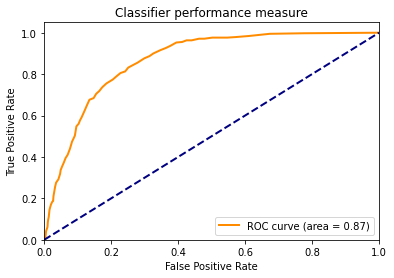
\includegraphics[width=\textwidth]{Images/Models/ROC_RandomForestV1.png}
    \caption{Receiver Operating Characteristic for initially trained classification model.}
    \label{fig:ROC_RandomForestV1}
\end{figure}

\begin{figure}[h]
    \centering
    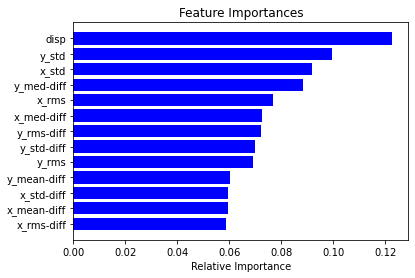
\includegraphics[width=\textwidth]{Images/Models/FI_RandomForestV1.png}
    \caption{Relative feature importances for initially trained classification model.}
    \label{fig:FI_RandomForestV1}
\end{figure}